\section{Functional MRI}
\label{sec:fmri}
\Gls{fMRI} using \gls{BOLD} contrast is the indispensable non-invasive method to investigate the brain function and organization. In the brain, there is an intimate connection between the brain and vasculature called the neurovascular coupling\cite{iadecolaNeurovascularUnitComing2017} to meet the local and high energy demand as shown in \cref{fig:BBB_microscopy}. The neuronal activity increases the local perfusion there by increasing the blood oxygenation, blood volume and blood flow. This process is detected as relative signal increase in a dynamic measurement as \gls{BOLD} effect\cite{ogawaBrainMagneticResonance1990} as the oxygenated blood has much higher $T_2^*$ than the deoxygenated blood. The \gls{BOLD}-\gls{fMRI} experiments are predominately performed using \gls{GE} sequences with a fast \gls{EPI} readout\cite{mansfieldMultiplanarImageFormation1977}. The spatio-temporal resolution of fMRI methods are limited due to the low intrinsic sensitivity of \gls{MRI} and relatively small signal change of 1-5\% at 3T. The typical spatial resolution of the fMRI studies at 3T is about 2-3 mm\cite{bollmannNewAcquisitionTechniques2021}. 

\begin{figure}[H]
	\centering
	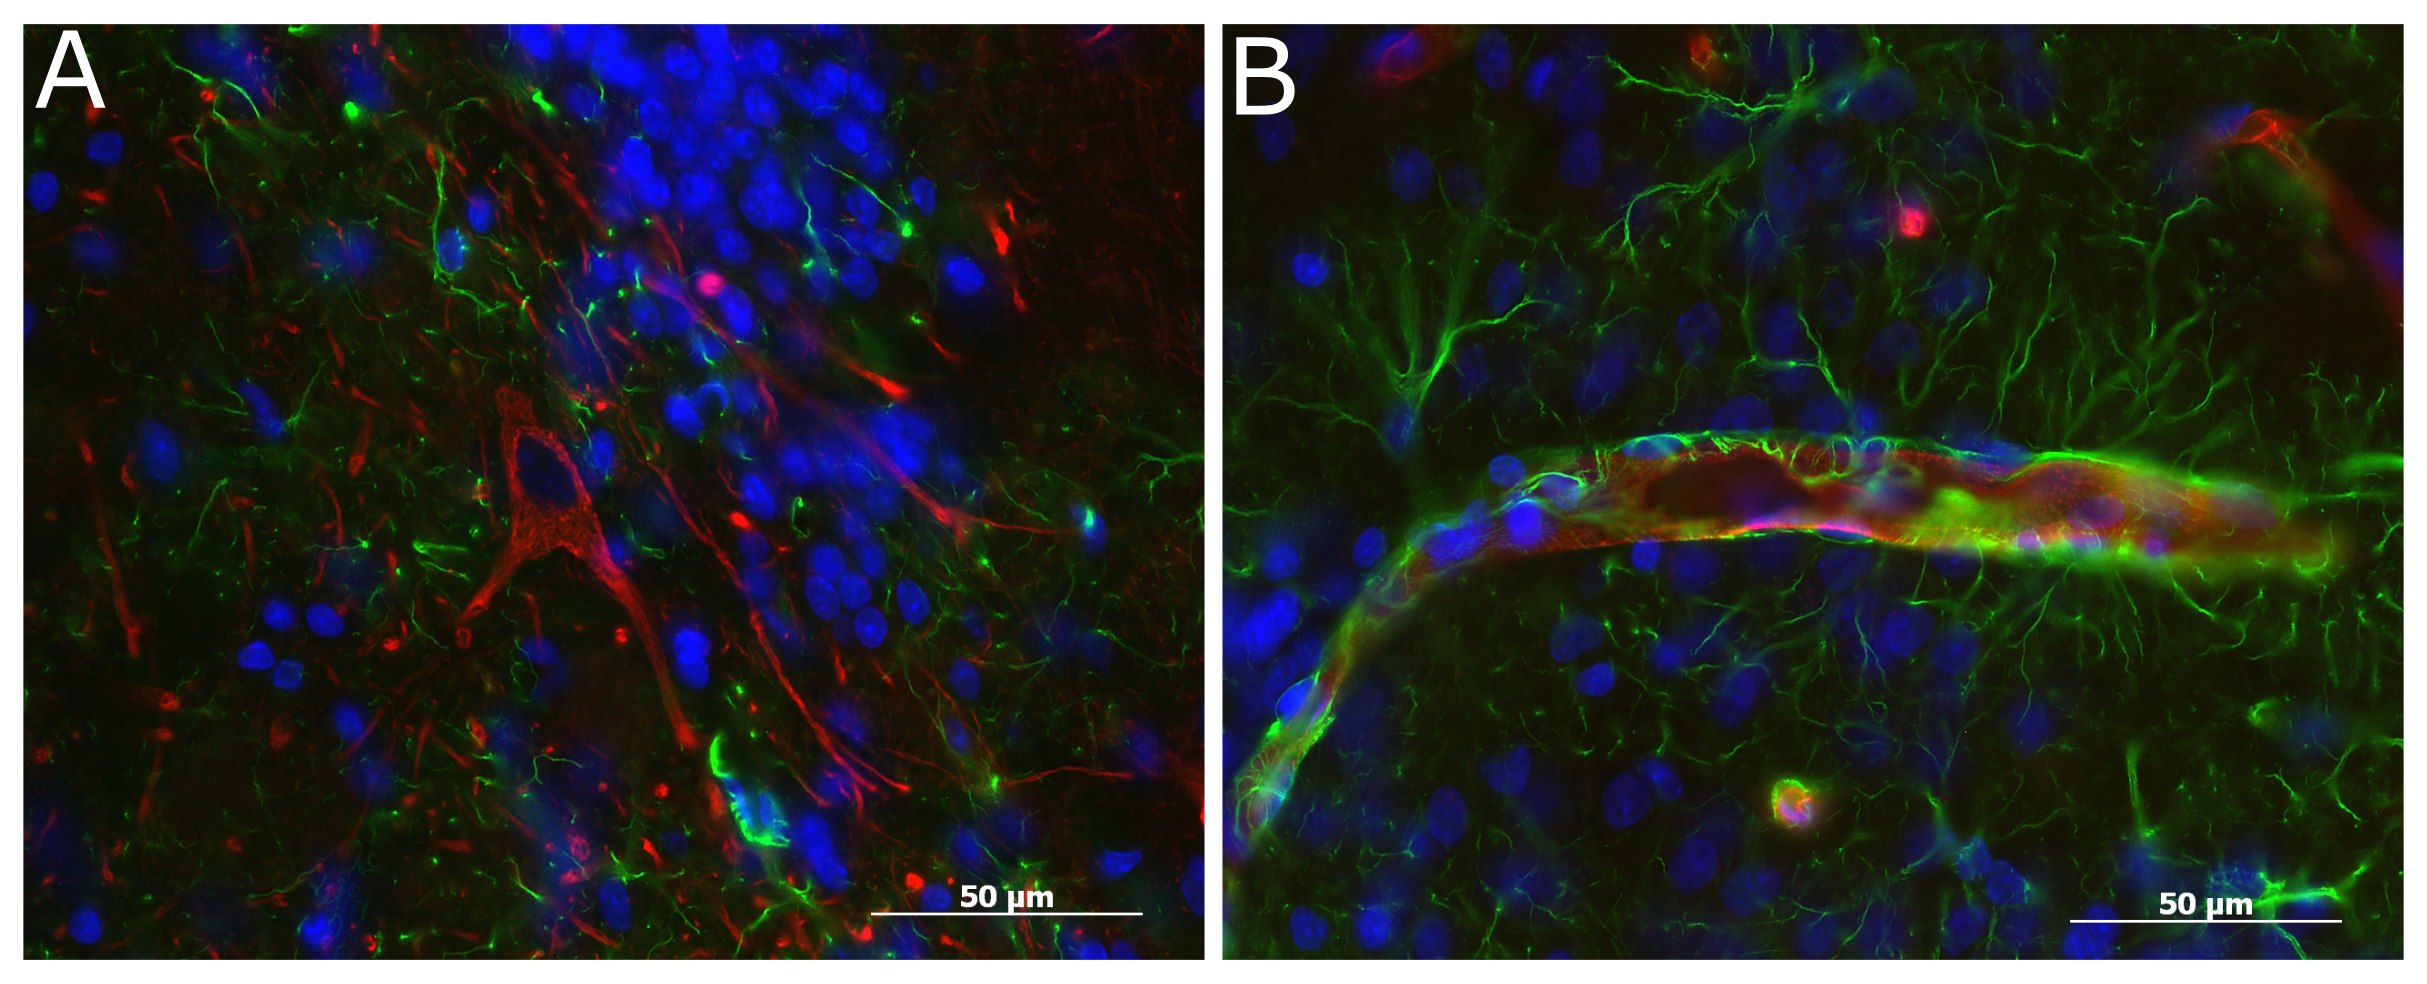
\includegraphics[width=1.0\textwidth]{graphics/BBB_microscopy.png}
	\caption{Immunofluorescence  microscopy showing cellular organization of a rat cortex. A) neuronal cell body, axons and dendrites in red(NF200 antibody), cytoskeleton of astrocytes in green (GFAP antibody), cell nuclei in blue (DAPI straining) B) endothelial cells of micro-vessel in red (RECA antibody), astrocytes processes around the blood vessel to regulate the flow in green (GFAP antibody), cell nuclei in blue (DAPI staining). (Photo credits: Gary Brook, Vishnu Mohandas, Praveen Iyyappan Valsala)}
	\label{fig:BBB_microscopy}
\end{figure}

Functional studies have progressively increased in complexity to investigate microscopic neuronal circuits involving individual cortical layers\cite{lawrenceLaminarFMRIApplications2019} and  columnar structures\cite{yacoubHighfieldFMRIUnveils2008}. Historically, investigations at such spatial scales were feasible only through electrophysiological approaches employing implanted electrode arrays, thereby restricting experimentation to animal models. Several synergistic hardware and methodological developments have pushed the boundaries of the human \gls{fMRI}. Especially, \gls{UHF} MRI scanners ($\geq 7T$) now enable \gls{fMRI} investigations at sub-millimeter resolution because of the supra-linear increase of \gls{SNR}\cite{pohmannSignaltonoiseRatioMR2016} and the significantly higher susceptibility-related $T_2^*$ contrast with the field strengths\cite{polimeniNeuroimagingUltrahighField2018}. Additionally, other hardware advances such as high-performance gradients, RF arrays with large number of receive elements, and temporal field monitoring systems\cite{barmetSpatiotemporalMagneticField2008} improved the spatio-temporal resolution and image quality.   

At the same time, new methodological approaches are enhancing the specificity of \gls{fMRI} methods. While conventional \gls{GE}-\gls{BOLD} remain dominant for their high sensitivity, its strong macrovascular contributions and the image distortions are problematic for high resolution studies, especially at \gls{UHF}.
Therefore, 

In particular, \gls{SE}-like methods such as \gls{SE}-\gls{EPI}\cite{yacoubSpinechoFMRIHumans2003,buddeFunctionalMRIHuman2014}, \gls{bSSFP}\cite{schefflerHighresolutionMappingNeuronal2016} and \gls{GRASE}\cite{kemperSubmillimeterT2Weighted2015} for making \gls{BOLD} contrast selective to smaller vessels like capillaries, thereby more closer to the neuronal activations.


BOLD contrast is the result of intra-voxel dephasing of water protons in the vicinity of deoxygenated blood due to neuronal activity. It has two main components namely 1) static dephasing regime which dominates in the large blood vessels where diffusion lengths are negligible and 2) dynamic averaging regime dominates in the small vessel where diffusion lengths are appreciable [13], [3]. As all the static dephasing are refocused in case of spin echo (SE), in SE-BOLD contrast only the latter effect dominates. Therefore, SE-BOLD contrast can localize neuronal activity at higher precision i.e. near capillary network and suppress the deoxygenated blood in the following macro vasculature like draining veins.


, VASO \cite{huberNonBOLDContrastLaminar2019}, and arterial spin labeling provide finer localization of neuronal activity by emphasizing small-vessel responses or blood volume and flow changes. These techniques complement UHF imaging by trading some sensitivity for sharper spatial precision, thereby narrowing the gap between observed hemodynamic signals and true neuronal events.

\subsection{bSSFP BOLD}
After the Ogawa et al.\cite{ogawaBrainMagneticResonance1990} reported measuring brain function with susceptibility changes in the blood in 1990, the first \gls{bSSFP} \gls{fMRI} application was reported only in 2001 \cite{schefflerDetectionBOLDChanges2001}. The initial methods\cite{schefflerDetectionBOLDChanges2001,millerFunctionalBrainImaging2003} mainly capitalized on the frequency sensitivity of the \gls{bSSFP} to detect \gls{BOLD} changes in the stopband. In 2005, Bowen et al. \cite{bowenHighFieldBalancedSSFP2005,bowenHighFieldBalancedSSFP2006} reported the first passband bSSFP and suggests its lower sensitivity to large draining veins because of its spin-echo properties\cite{schefflerTrueFISPGradientechoSpinecho2003}. 

\begin{figure}[H]
	\centering
	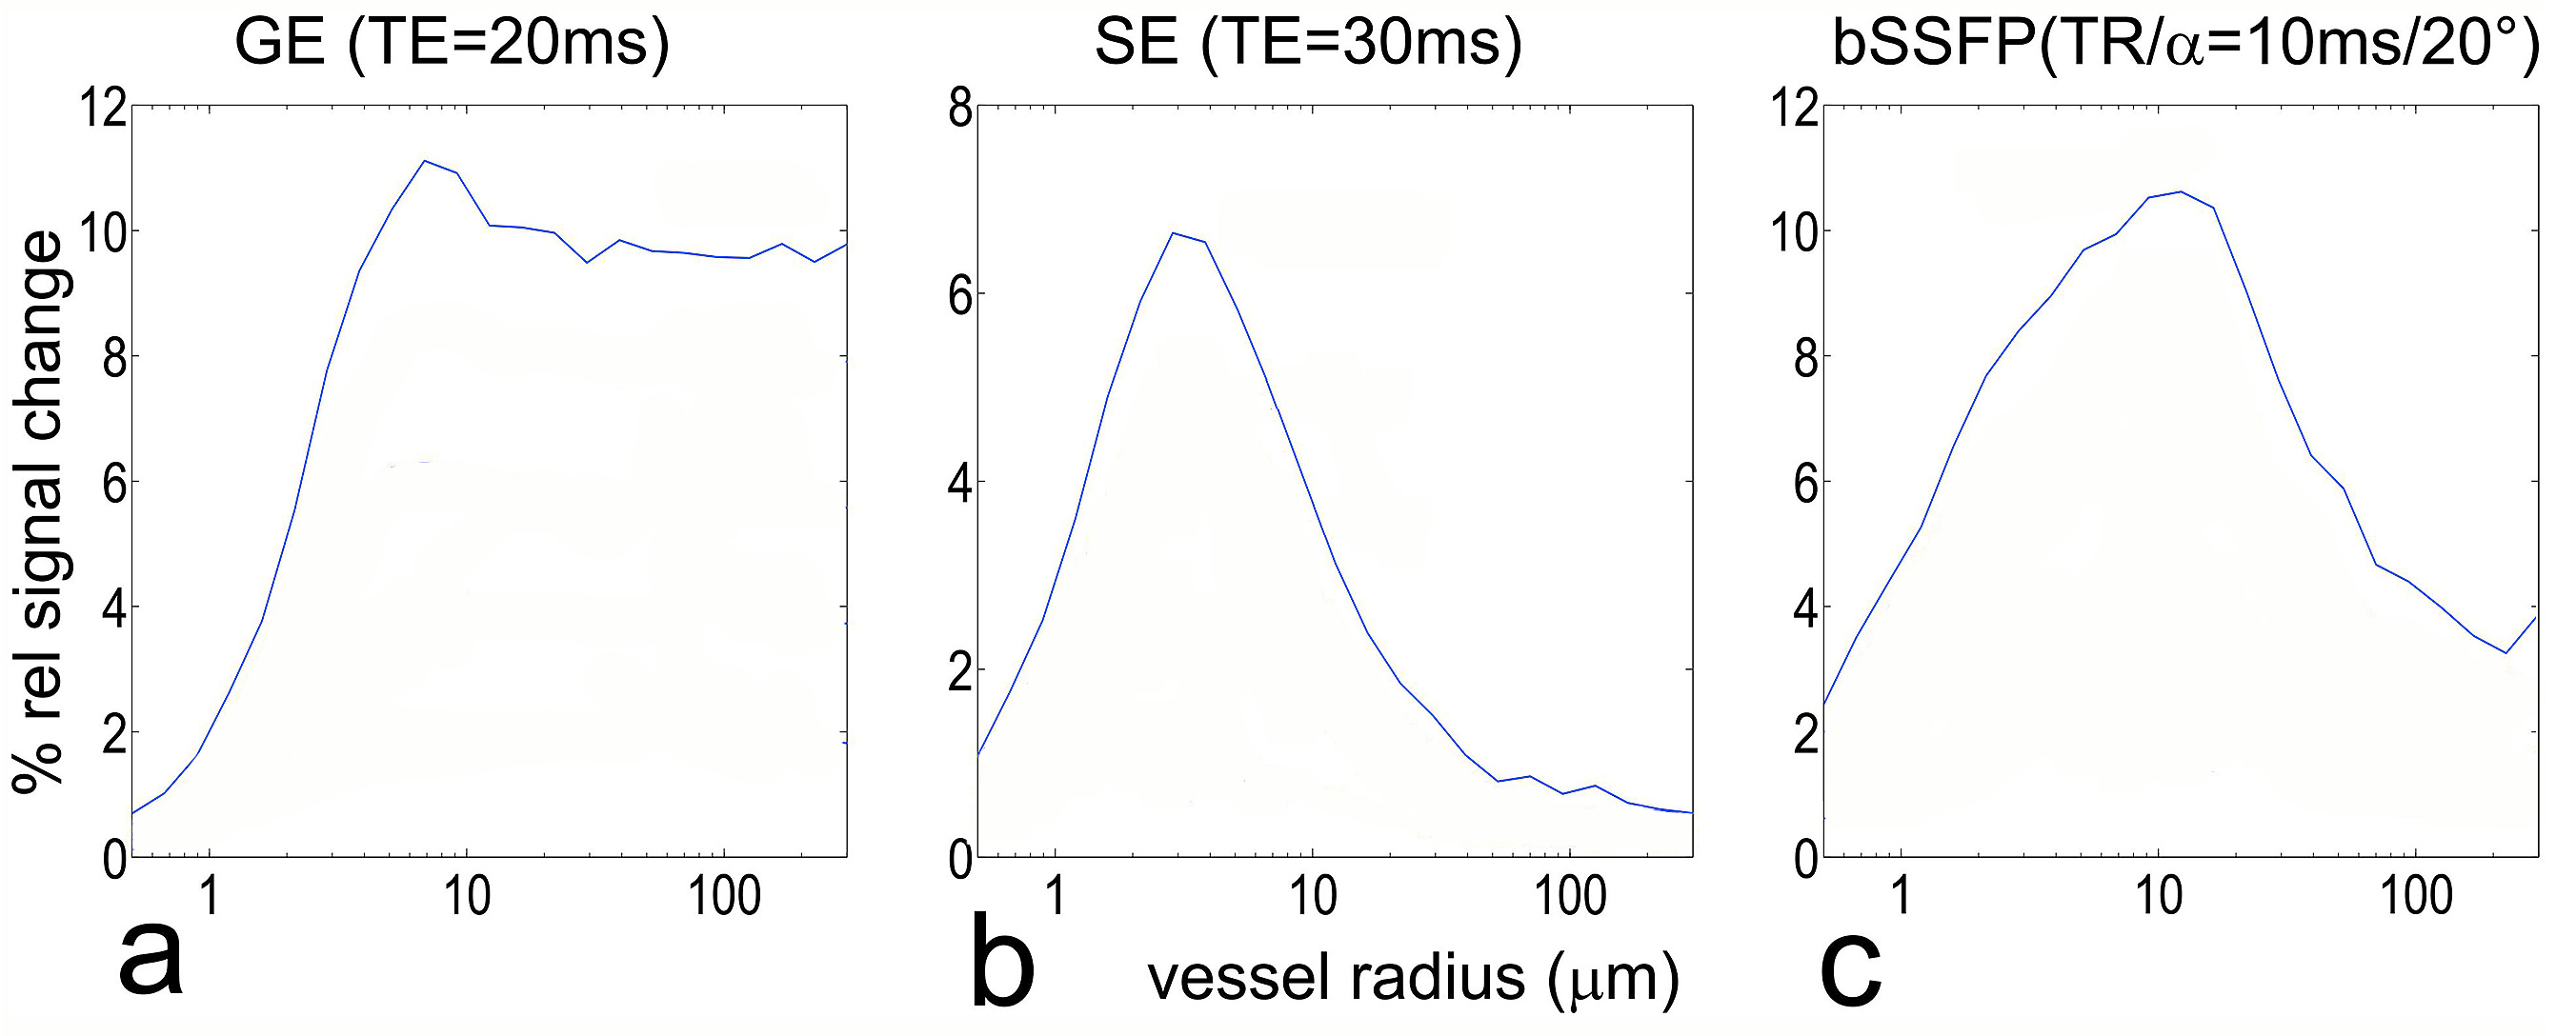
\includegraphics[width=1.0\textwidth]{graphics/fmi_bssfp_BVF5.png}
	\caption{Simulated BOLD related signal change of \gls{GE}, \gls{SE} and \gls{bSSFP} as a function of vessel (randomly oriented cylinders) for 5\% blood volume fraction at 9.4 T. Both \gls{SE} and \gls{bSSFP} show similarly suppressed BOLD signal change for large vessel radius of $\ge 100\,\mu m$. Adapted from Baez-Yanez et al.~\cite{baez-yanezImpactVesselSize2017}}
	\label{fig:vesselSize}
\end{figure}





However, the BOLD signal change with \gls{bSSFP} acquisition is only half of that of the GRE-BOLD\cite{schefflerHighresolutionMappingNeuronal2016}. 




The
- For this gain in specificity, several SE-BOLD methods are developed like SE-EPI, RASER, GRASE, SSFP and many more[12]. Among these methods, balanced steady state free precision (bSSFP) is well suited for UHF-fMRI because of its low SAR requirement and high temporal resolution [17], [18], [11].
Contrary to its name, the BOLD contrast, in addition to oxygen metabolism, also depends on blood flow rate (CBF) and cerebral blood volume(CBV) changes [6]. Together with the SE methods, the methods sensitive to these changes are also investigated to increase the specificity of fMRI. Vascular space occupancy (VASO)-dependent fMRI measures neuronal activity by tracking the CBV changes. It utilizes the fact that blood and tissues has different T1 relaxation times and nulls the signal from the blood using a sophisticated inversion recovery sequence [9]. In CBF-dependent BOLD technique mainly uses Arterial spin labeling methods (ASL) to measure neuronal activity related perfusion changes. The spins in the in-flowing blood are labeled by either inversion or saturation and perfusion is measured at the region of interest by the corresponding signal drop [15]. Similar to the SE-BOLD methods, these methods also has poor sensitivity and longer acquisition duration compared to GRE-BOLD methods.

\subsection{things to include}

high field fmri(VASO)
BOLD effects (spin echo)

acquistion speed of ssfp 